\section{Cimentaciones profundas} % (fold)
\label{sec:cimentaciones_profundas}

\begin{mybox}{Pilotes}
Es la máxima presión que puede sufrir el terreno bajo la cimentación
\tcbsubtitle{\emph{CPI 4}}
	\begin{enumerate}
		\item Avance tubería con cuchare o trépano
		\item Empotramiento del pilote
		\item Hormigonado y extracción de la tubería
	\end{enumerate}
\tcbsubtitle{\emph{CPI 7}}
	\begin{enumerate}
		\item Avance de la perforación con el auger
		\item Hormigonado
	\end{enumerate}
	\begin{myrem}[Restricción]
		El terreno ha de tener cierta cohesión
	\end{myrem}
\tcbsubtitle{\emph{CPI 8 (barrena continua)}}
	\begin{enumerate}
		\item Introducimos la barrena a rotación hasta el fondo (donde se quiere llegar)
		\item Se hormigona mientras se va quitando la barrena
		\item Introducción de la armadura en el hormigón fresco
	\end{enumerate}
	\begin{myrem}[Armaduras]
		Suelen trabajar a compresión, luego si la armadura no es más corta no tiene porque ser problemático.
	\end{myrem}
\tcbsubtitle{\emph{CPI 3 (hincado)}}
	\begin{enumerate}
		\item Hincado
		\item Formación del bulbo
		\item Hormigonado y extracción de la tuberia
	\end{enumerate}
\end{mybox}

\begin{figure}[H]
		\centering
		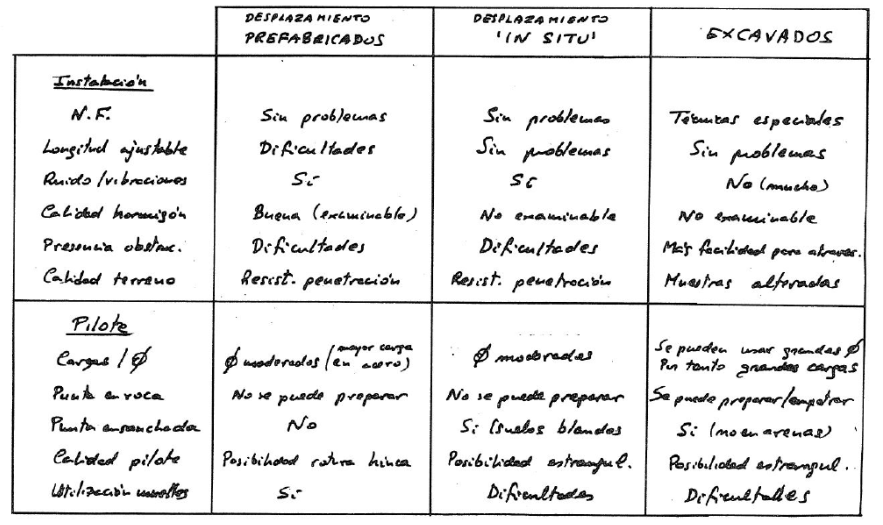
\includegraphics[width=\textwidth]{img/compar}
		\caption{Comparación de los distintos métodos}
		\label{fig:compar}
\end{figure}

\begin{mybox}{Método Delft}
	\begin{ldef}[Delft]
		Permite calcular la resistencia en punta de un pilote
	\end{ldef}

	La resistencia no es uniforme, así pues solemos estimar un único valor medio de la distribución.

	\tcbsubtitle{\emph{Procedimiento}}

	Se definen 3 zonas, de menor a mayor profundidad y se cálcula
	\begin{equation}
		\begin{cases}
			q_c = \frac{(q_c)_{I}+(q_c)_{II}}{2}, &\text{ if }(q_c)_{III} >(q_c)_{II} \\
			q_c = \frac{(q_c)_{I}+\frac{(q_c)_{II}+(q_c)_{III}}{2}}{2}, &\text{ if }(q_c)_{III} \leq(q_c)_{II}
		\end{cases}
	\end{equation}
\end{mybox}

% section cimentaciones_profundas (end)